% Medio anisótropo: J no es paralelo a E (libro cap. 4.1)
\documentclass[border=4pt]{standalone}
\usepackage{amsmath}
\usepackage{tikz}
\usetikzlibrary{arrows.meta, calc}
\begin{document}
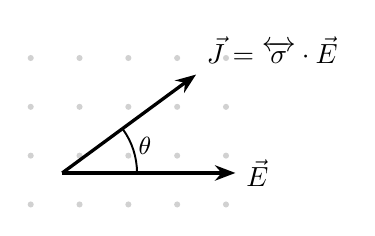
\begin{tikzpicture}[>={Stealth[length=2.6mm]}, line width=0.7pt]
  % red cristalina de fondo (puntos)
  \foreach \i in {0,...,4}{\foreach \j in {0,...,3}{
    \fill[black!18] (\i*0.62,\j*0.62) circle (1.1pt);}}
  \coordinate (O) at (0.4,0.4);
  \draw[->, line width=1.2pt] (O)--($(O)+(2.2,0)$) node[right]{$\vec E$};
  \draw[->, line width=1.2pt] (O)--($(O)+(1.7,1.25)$) node[above right]{$\vec J=\overleftrightarrow{\sigma}\cdot\vec E$};
  % ángulo de desvío
  \draw (O)+(0.95,0) arc (0:36:0.95);
  \node at ($(O)+(1.05,0.34)$) {\small$\theta$};
\end{tikzpicture}
\end{document}
